% =============================================================================
%  SOFTWARE REQUIREMENTS SPECIFICATION (SRS)
%  Real-Time Collaborative Programming Extension for Visual Studio Code
%  IEEE 830 / ISO/IEC/IEEE 29148:2018 Compliant
% =============================================================================
\documentclass[12pt, a4paper, oneside]{article}

% --- Core Packages ---
\usepackage[utf8]{inputenc}
\usepackage[T1]{fontenc}
\usepackage{lmodern}
\usepackage[margin=2.5cm]{geometry}
\usepackage{setspace}
\onehalfspacing

% --- Graphics and Diagrams ---
\usepackage{tikz}
\usetikzlibrary{
  shapes.geometric, arrows.meta, positioning, calc,
  decorations.pathmorphing, fit, backgrounds, shadows,
  matrix, chains, patterns
}
\usepackage{pgfplots}
\pgfplotsset{compat=1.18}

% --- Tables and Lists ---
% --- Tables and Lists ---
\usepackage{booktabs}
\usepackage{tabularx}
\usepackage{ragged2e}
\newcolumntype{Y}{>{\RaggedRight\arraybackslash}X}
\usepackage{longtable}
\usepackage{enumitem}
\usepackage{multirow}

% --- Formatting ---
\usepackage{xcolor}
\usepackage{hyperref}
\usepackage{fancyhdr}
\usepackage{titlesec}
\usepackage{tocloft}
\usepackage{float}
\usepackage{caption}
\usepackage{amsmath, amssymb}

% --- Color Palette (Muted Professional) ---
\definecolor{primaryblue}{HTML}{2C3E50}
\definecolor{accentlink}{HTML}{3498DB}
\definecolor{darkbg}{HTML}{2C3E50}
\definecolor{accentgreen}{HTML}{27AE60}
\definecolor{warnorange}{HTML}{E67E22}
\definecolor{lightgray}{HTML}{ECF0F1}
\definecolor{sectioncolor}{HTML}{2C3E50}
\definecolor{crdt}{HTML}{8E44AD}
\definecolor{ot}{HTML}{16A085}
\definecolor{client}{HTML}{2980B9}
\definecolor{server}{HTML}{C0392B}
\definecolor{broker}{HTML}{D35400}

% --- Header / Footer ---
\pagestyle{fancy}
\fancyhf{}
\fancyhead[L]{\small\textcolor{sectioncolor}{SRS --- VS Code Live Share Extension}}
\fancyhead[R]{\small\textcolor{sectioncolor}{v1.0}}
\fancyfoot[C]{\thepage}
\renewcommand{\headrulewidth}{0.4pt}

% --- Section Styling ---
\titleformat{\section}
  {\Large\bfseries\color{sectioncolor}}{\thesection}{1em}{}[\vspace{-0.5em}\textcolor{primaryblue}{\rule{\textwidth}{1.5pt}}]
\titleformat{\subsection}
  {\large\bfseries\color{sectioncolor}}{\thesubsection}{1em}{}
\titleformat{\subsubsection}
  {\normalsize\bfseries\color{sectioncolor}}{\thesubsubsection}{1em}{}

% --- Custom Commands ---
\newcommand{\reqid}[1]{\texttt{\textcolor{primaryblue}{#1}}}
\newcommand{\metric}[1]{\textbf{\textcolor{accentgreen}{#1}}}
\newcommand{\warn}[1]{\textbf{\textcolor{warnorange}{#1}}}

% --- TikZ Styles ---
\tikzset{
  component/.style={
    rectangle, rounded corners=6pt, minimum width=3.2cm, minimum height=1.2cm,
    align=center, font=\small\bfseries, draw=#1!70, fill=#1!12,
    drop shadow={shadow xshift=1pt, shadow yshift=-1pt, opacity=0.15}
  },
  connector/.style={
    -Stealth, thick, color=#1!70
  },
  note/.style={
    rectangle, rounded corners=3pt, font=\scriptsize, fill=yellow!15,
    draw=yellow!50!black, text width=2.8cm, align=center
  },
  brace/.style={
    decorate, decoration={brace, amplitude=6pt, raise=2pt}
  }
}

\begin{document}

% ===================== TITLE PAGE =====================
\begin{titlepage}
\centering
\vspace*{1.5cm}

\begin{center}
{\Huge\bfseries\color{sectioncolor} Software Requirements Specification}
\end{center}

\vspace{1.2cm}
{\LARGE\bfseries\color{primaryblue} Real-Time Collaborative Programming Extension\\[4pt]
for Visual Studio Code}

\vspace{0.8cm}
{\large (VS Code Live Share Clone)}

\vspace{2cm}
\begin{tabular}{rl}
  \textbf{Document Version:} & 1.0 \\
  \textbf{Date:}             & \today \\
  \textbf{Standard:}         & IEEE 830 / ISO/IEC/IEEE 29148:2018 \\
  \textbf{Course:}           & Software Engineering --- 6\textsuperscript{th} Semester \\
  \textbf{Institution:}      & IIIT Hyderabad \\
\end{tabular}

\vfill
{\small\color{gray} Collaborative Software Engineering Project --- Internal Documentation}
\end{titlepage}

% ===================== REVISION HISTORY =====================
\newpage
\section*{Revision History}
\begin{table}[H]
\centering
\begin{tabularx}{\textwidth}{c c c X}
\toprule
\textbf{Version} & \textbf{Date} & \textbf{Author} & \textbf{Description} \\
\midrule
0.1 & 2026-03-15 & Team & Initial requirements gathering \\
0.5 & 2026-03-25 & Team & Architectural evaluation and NFR quantification \\
1.0 & 2026-04-05 & Team & Complete SRS with ATAM scenarios \\
\bottomrule
\end{tabularx}
\end{table}

\tableofcontents
\newpage

% ===================== 1. INTRODUCTION =====================
\section{Introduction}

\subsection{Purpose}
This SRS documents the functional and non-functional requirements for the \textbf{CollabCode} extension. It provides the technical basis for development and evaluation.

The requirements follow standard specifications to ensure all project goals are traceable and measurable.

\subsection{Scope}
The system, hereafter referred to as \textbf{CollabCode}, shall enable $N \geq 2$ developers to simultaneously edit the same codebase in real time from independent VS Code instances, with automatic conflict resolution guaranteeing \textbf{eventual consistency} across all replicas.

\begin{table}[H]
\centering
\caption{Project Scope Summary}
\begin{tabularx}{\textwidth}{l X}
\toprule
\textbf{Attribute} & \textbf{Value} \\
\midrule
Product Name       & CollabCode \\
Platform           & VS Code Extension (Electron / Node.js) \\
Max Concurrent Users per Session & 8 (target), 15 (stretch goal) \\
Supported Languages & Language-agnostic (operates on plain text) \\
Delivery Format    & \texttt{.vsix} package via VS Code Marketplace \\
Development Duration & 12 weeks (3 sprints $\times$ 4 weeks) \\
Team Size          & 4--6 developers \\
\bottomrule
\end{tabularx}
\end{table}

\subsection{Definitions, Acronyms, and Abbreviations}
\begin{table}[H]
\centering
\begin{tabularx}{\textwidth}{l X}
\toprule
\textbf{Term} & \textbf{Definition} \\
\midrule
CRDT   & Conflict-free Replicated Data Type --- data structures that merge concurrent updates automatically \\
OT     & Operational Transformation --- algorithm that transforms concurrent operations to preserve intent \\
Replica & Local copy of the shared document state at each client node \\
Causal Consistency & Consistency model preserving cause-and-effect ordering of events \\
Walking Skeleton & Minimal end-to-end implementation validating core architectural risks \\
ATAM   & Architecture Tradeoff Analysis Method \\
NFR    & Non-Functional Requirement \\
E2E    & End-to-End \\
P99    & 99\textsuperscript{th} percentile latency \\
\bottomrule
\end{tabularx}
\end{table}

\subsection{References}
\begin{enumerate}[label={[R\arabic*]}]
  \item IEEE Std 830-1998, \textit{Recommended Practice for SRS}.
  \item ISO/IEC/IEEE 29148:2018, \textit{Systems and software engineering --- Life cycle processes --- Requirements engineering}.
  \item M.~Kleppmann and A.~R.~Beresford, ``A Conflict-Free Replicated JSON Datatype,'' \textit{IEEE TPDS}, vol.~28, no.~10, 2017.
  \item C.~Sun and C.~Ellis, ``Operational Transformation in Real-Time Group Editors,'' \textit{Proc. ACM CSCW}, 1998.
  \item ICSE 2025, ``Understanding Real-time Collaborative Programming: a Study of Visual Studio Live Share.''
  \item L.~Bass, P.~Clements, and R.~Kazman, \textit{Software Architecture in Practice}, 4th ed., Addison-Wesley, 2021.
\end{enumerate}

% ===================== 2. OVERALL DESCRIPTION =====================
\section{Overall Description}

\subsection{Product Perspective}
CollabCode operates as a \textbf{VS Code extension} that injects a collaboration layer atop the Monaco editor. It communicates with a lightweight relay server over secure WebSocket channels. The system follows a \textbf{multi-leader replication} topology where each IDE instance is an autonomous leader that applies edits locally and asynchronously replicates them to peers.

% --- HIGH-LEVEL ARCHITECTURE DIAGRAM ---
\begin{figure}[H]
\centering
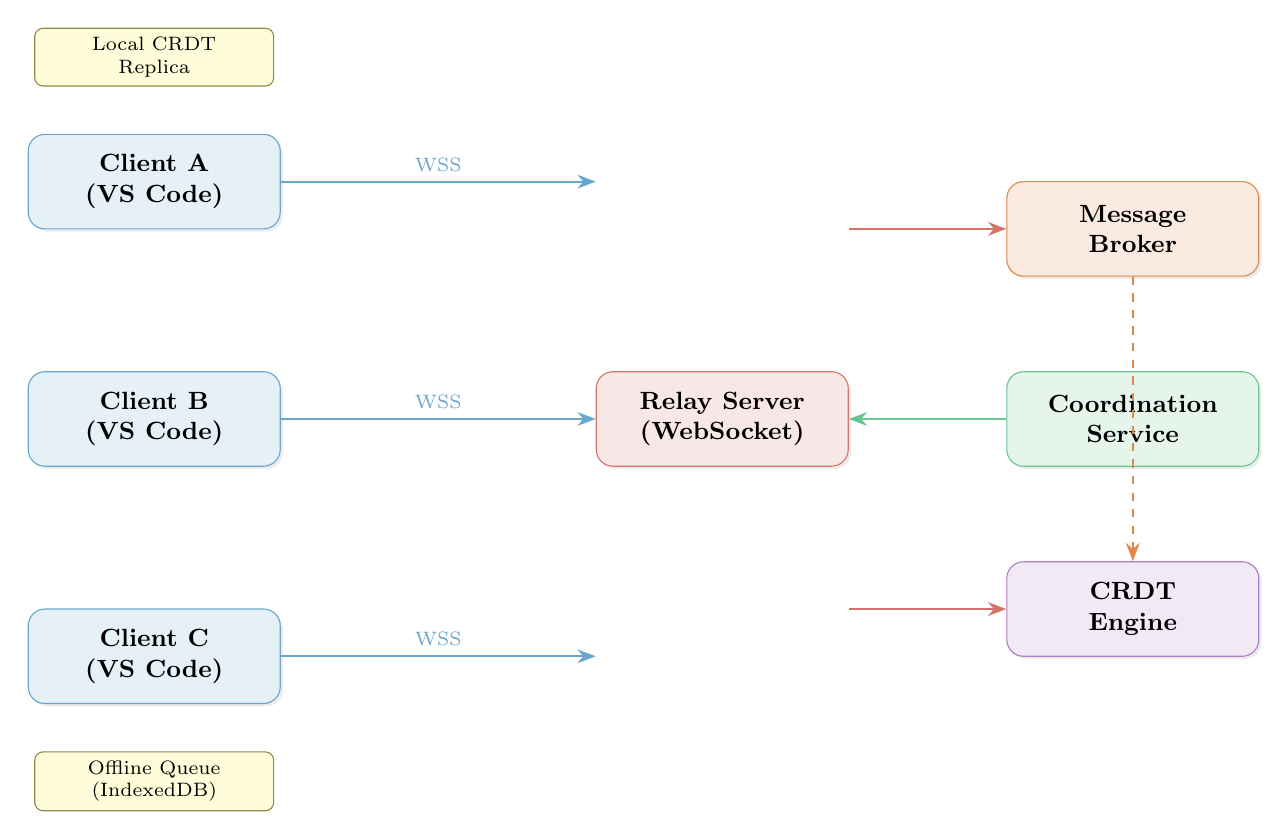
\begin{tikzpicture}[node distance=1.8cm and 2.5cm]

  % Clients
  \node[component=client] (c1) {Client A\\(VS Code)};
  \node[component=client, below=of c1] (c2) {Client B\\(VS Code)};
  \node[component=client, below=of c2] (c3) {Client C\\(VS Code)};

  % Server cluster
  \node[component=server, right=4cm of c2] (relay) {Relay Server\\(WebSocket)};
  \node[component=broker, above right=1.2cm and 2cm of relay] (broker) {Message\\Broker};
  \node[component=crdt, below right=1.2cm and 2cm of relay] (crdt) {CRDT\\Engine};

  % Coordination
  \node[component=accentgreen, right=2cm of relay] (coord) {Coordination\\Service};

  % Connections
  \draw[connector=client] (c1.east) -- node[above, font=\scriptsize, sloped]{WSS} (relay.west |- c1.east);
  \draw[connector=client] (c2.east) -- node[above, font=\scriptsize]{WSS} (relay.west);
  \draw[connector=client] (c3.east) -- node[above, font=\scriptsize, sloped]{WSS} (relay.west |- c3.east);

  \draw[connector=server] (relay.east |- broker.west) -- (broker.west);
  \draw[connector=server] (relay.east |- crdt.west) -- (crdt.west);
  \draw[connector=accentgreen] (coord.west) -- (relay.east);
  \draw[connector=broker, dashed] (broker.south) -- (crdt.north);

  % Labels
  \node[note, above=0.6cm of c1] {Local CRDT\\Replica};
  \node[note, below=0.6cm of c3] {Offline Queue\\(IndexedDB)};

\end{tikzpicture}
\caption{High-Level System Architecture --- Multi-Leader Replication Topology}
\label{fig:arch}
\end{figure}

\subsection{System Stakeholders}

\begin{table}[H]
\centering
\caption{Stakeholder Registry}
\begin{tabularx}{\textwidth}{l l X l}
\toprule
\textbf{ID} & \textbf{Role} & \textbf{Concerns} & \textbf{Priority} \\
\midrule
SH-01 & End Users (Developers) & Latency $<200$\,ms, zero data loss, intuitive UX & Critical \\
SH-02 & Instructors / Evaluators & Architectural rigor, empirical metrics, IEEE compliance & Critical \\
SH-03 & Dev Team (Practitioners) & Maintainability, testability, clean API boundaries & High \\
SH-04 & Team Lead / PM & Sprint velocity, risk mitigation, milestone delivery & High \\
SH-05 & IT / Ops & Deployment simplicity, monitoring, security posture & Medium \\
\bottomrule
\end{tabularx}
\end{table}

\subsection{Product Functions (Summary)}
\begin{enumerate}
  \item \textbf{Session Management} --- Create, join, and leave collaborative sessions via unique session tokens.
  \item \textbf{Real-Time Co-Editing} --- Simultaneous multi-cursor editing with character-level granularity.
  \item \textbf{Conflict Resolution} --- Automatic CRDT-based merge of concurrent operations.
  \item \textbf{Presence Awareness} --- Live cursors, selections, and participant indicators.
  \item \textbf{Shared Terminal} --- Read-only shared terminal output for the session host's terminal.
  \item \textbf{File Explorer Sync} --- Synchronized view of the project file tree.
  \item \textbf{Chat and Annotations} --- In-editor text chat and line-level annotations.
\end{enumerate}

\subsection{User Classes and Characteristics}
\begin{table}[H]
\centering
\caption{User Classes}
\begin{tabularx}{\textwidth}{l c c X}
\toprule
\textbf{User Class} & \textbf{Frequency} & \textbf{Technical Level} & \textbf{Primary Goals} \\
\midrule
Session Host    & Daily   & Intermediate--Expert & Share workspace, manage permissions \\
Session Guest   & Daily   & Beginner--Expert     & Navigate, edit, and debug collaboratively \\
Observer (Read-Only) & Weekly & Any            & Review code, provide feedback \\
\bottomrule
\end{tabularx}
\end{table}

\subsection{Operating Environment}
\begin{itemize}
  \item \textbf{Client:} VS Code $\geq$1.85, Node.js $\geq$18 LTS, Windows/macOS/Linux.
  \item \textbf{Server:} Node.js 20 LTS, Docker-containerized, deployable on any cloud provider.
  \item \textbf{Network:} TCP/IP with TLS 1.3; WebSocket (RFC 6455) over HTTPS.
  \item \textbf{Minimum Bandwidth:} 256\,Kbps per client for text-only sessions.
\end{itemize}

\subsection{Assumptions and Dependencies}
\begin{enumerate}
  \item Users have stable internet connectivity ($\geq$256\,Kbps, $\leq$150\,ms RTT to relay).
  \item VS Code Extension API remains backward-compatible through development cycle.
  \item The CRDT library (\texttt{Yjs} or \texttt{Automerge}) is used as a proven foundation.
  \item The relay server will be hosted on a single cloud region for the prototype phase.
\end{enumerate}

% ===================== 3. FUNCTIONAL REQUIREMENTS =====================
\section{Specific Requirements --- Functional}

\subsection{Session Management}

\begin{table}[H]
\centering
\caption{Session Management Requirements}
\begin{tabularx}{\textwidth}{l l X l}
\toprule
\textbf{ID} & \textbf{Name} & \textbf{Description} & \textbf{Priority} \\
\midrule
\reqid{FR-SM-01} & Create Session & The host shall generate a unique 128-bit session token and initialize a CRDT document state on the relay server within \metric{$\leq$500\,ms}. & Must \\
\reqid{FR-SM-02} & Join Session & A guest shall connect to an active session via token. Handshake and full state sync shall complete in \metric{$\leq$2\,s} for documents $\leq$50\,KB. & Must \\
\reqid{FR-SM-03} & Leave Session & Disconnection shall be detected within \metric{$\leq$3\,s} via heartbeat timeout (interval = 1\,s). Replica state shall be preserved for \metric{60\,s} for reconnection. & Must \\
\reqid{FR-SM-04} & Permission Roles & Host shall assign roles: \textit{Owner}, \textit{Editor}, \textit{Read-Only}. Role changes propagate in \metric{$\leq$500\,ms}. & Should \\
\reqid{FR-SM-05} & Session Persistence & Session metadata (participant list, timestamp log) shall persist for \metric{72\,hours} after session end. & Could \\
\bottomrule
\end{tabularx}
\end{table}

\subsection{Real-Time Co-Editing}

\begin{table}[H]
\centering
\caption{Co-Editing Requirements}
\begin{tabularx}{\textwidth}{l l X l}
\toprule
\textbf{ID} & \textbf{Name} & \textbf{Description} & \textbf{Priority} \\
\midrule
\reqid{FR-CE-01} & Local-First Edit & Every keystroke shall be applied to the local CRDT replica in \metric{$\leq$5\,ms} (local latency). & Must \\
\reqid{FR-CE-02} & Remote Sync & Local operations shall be broadcast to all peers; remote peers shall apply received operations in \metric{$\leq$200\,ms} E2E (P95). & Must \\
\reqid{FR-CE-03} & Conflict Resolution & Concurrent inserts/deletes at the same position shall be resolved deterministically by the CRDT merge function with \metric{100\%} convergence guarantee. & Must \\
\reqid{FR-CE-04} & Multi-File Support & The system shall support concurrent editing across \metric{$\leq$20} open files per session. & Should \\
\reqid{FR-CE-05} & Undo/Redo & Per-user undo/redo stack preserving only the local user's operations (selective undo). & Should \\
\bottomrule
\end{tabularx}
\end{table}

\subsection{Presence Awareness}

\begin{table}[H]
\centering
\caption{Presence Awareness Requirements}
\begin{tabularx}{\textwidth}{l l X l}
\toprule
\textbf{ID} & \textbf{Name} & \textbf{Description} & \textbf{Priority} \\
\midrule
\reqid{FR-PA-01} & Live Cursors & Each remote user's cursor position shall be displayed with a unique color and name label, updated at \metric{$\geq$10\,Hz}. & Must \\
\reqid{FR-PA-02} & Selection Highlight & Remote user selections shall be highlighted with a translucent overlay of the user's assigned color. & Must \\
\reqid{FR-PA-03} & Follow Mode & A ``Follow Participant'' mode shall scroll the local viewport to track a selected peer's cursor in real time. & Should \\
\reqid{FR-PA-04} & Participant List & A sidebar panel shall display all connected participants with status indicators (active / idle / disconnected). & Must \\
\bottomrule
\end{tabularx}
\end{table}

\subsection{Shared Terminal and Debugging}

\begin{table}[H]
\centering
\caption{Shared Terminal Requirements}
\begin{tabularx}{\textwidth}{l l X l}
\toprule
\textbf{ID} & \textbf{Name} & \textbf{Description} & \textbf{Priority} \\
\midrule
\reqid{FR-ST-01} & Terminal Sharing & Host may share terminal output as a read-only stream to guests. Terminal data throughput: \metric{$\leq$64\,KB/s}. & Should \\
\reqid{FR-ST-02} & Shared Debugging & Host may share an active debug session; guests observe breakpoints, call stack, and variable state. & Could \\
\bottomrule
\end{tabularx}
\end{table}

\subsection{Communication}

\begin{table}[H]
\centering
\caption{Communication Requirements}
\begin{tabularx}{\textwidth}{l l X l}
\toprule
\textbf{ID} & \textbf{Name} & \textbf{Description} & \textbf{Priority} \\
\midrule
\reqid{FR-CO-01} & Text Chat & In-editor chat panel supporting plain-text messages with \metric{$\leq$300\,ms} delivery latency. & Should \\
\reqid{FR-CO-02} & Code Annotations & Users may attach ephemeral comments to specific line ranges, visible to all participants. & Could \\
\bottomrule
\end{tabularx}
\end{table}

% ===================== 4. NON-FUNCTIONAL REQUIREMENTS =====================
\section{Specific Requirements --- Non-Functional}

\subsection{Performance Requirements}

% --- LATENCY BUDGET DIAGRAM ---
\begin{figure}[H]
\centering
\resizebox{0.9\textwidth}{!}{
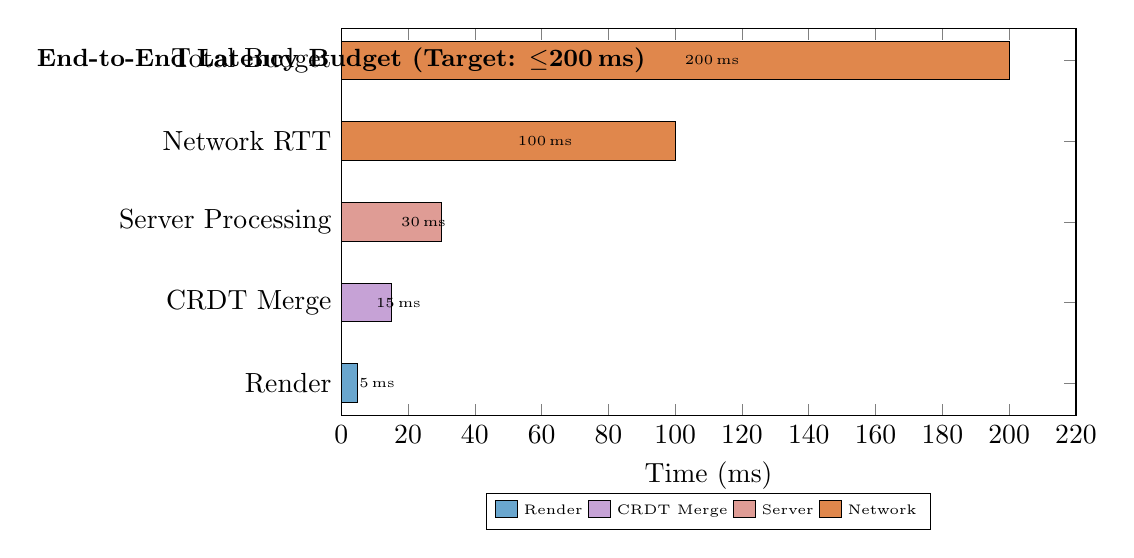
\begin{tikzpicture}
  \begin{axis}[
    title={\textbf{End-to-End Latency Budget (Target: $\leq$200\,ms)}},
    xbar stacked,
    xlabel={Time (ms)},
    symbolic y coords={Total Budget, Network RTT, Server Processing, CRDT Merge, Render},
    ytick=data,
    y dir=reverse,
    xmin=0, xmax=220,
    width=0.9\textwidth, height=6.5cm,
    bar width=14pt,
    legend style={at={(0.5,-0.2)}, anchor=north, legend columns=4, font=\tiny},
    nodes near coords={\pgfmathprintnumber\pgfplotspointmeta\,ms},
    nodes near coords style={font=\tiny, anchor=west},
    every axis title/.style={font=\small},
  ]
  \addplot[fill=client!70] coordinates {(5,Render) (0,CRDT Merge) (0,Server Processing) (0,Network RTT) (0,Total Budget)};
  \addplot[fill=crdt!50] coordinates  {(0,Render) (15,CRDT Merge) (0,Server Processing) (0,Network RTT) (0,Total Budget)};
  \addplot[fill=server!50] coordinates {(0,Render) (0,CRDT Merge) (30,Server Processing) (0,Network RTT) (0,Total Budget)};
  \addplot[fill=broker!70] coordinates {(0,Render) (0,CRDT Merge) (0,Server Processing) (100,Network RTT) (200,Total Budget)};
  \legend{Render, CRDT Merge, Server, Network}
  \end{axis}
\end{tikzpicture}
}
\caption{Latency Budget Allocation --- Performance Constraints}
\label{fig:latency}
\end{figure}

\begin{table}[H]
\centering
\caption{Quantified Performance Targets}
\begin{tabularx}{\textwidth}{l X c c}
\toprule
\textbf{ID} & \textbf{Metric} & \textbf{Target} & \textbf{Threshold} \\
\midrule
\reqid{NFR-P-01} & E2E sync latency (P95) & $\leq$150\,ms & $\leq$200\,ms \\
\reqid{NFR-P-02} & E2E sync latency (P99) & $\leq$200\,ms & $\leq$350\,ms \\
\reqid{NFR-P-03} & Local keystroke latency & $\leq$5\,ms & $\leq$16\,ms \\
\reqid{NFR-P-04} & State convergence time (8 users) & $\leq$500\,ms & $\leq$1\,s \\
\reqid{NFR-P-05} & Throughput (operations/sec/session) & $\geq$500 & $\geq$200 \\
\reqid{NFR-P-06} & Session creation time & $\leq$500\,ms & $\leq$1\,s \\
\reqid{NFR-P-07} & Initial state sync ($\leq$50\,KB doc) & $\leq$2\,s & $\leq$4\,s \\
\reqid{NFR-P-08} & Memory per client (idle session) & $\leq$80\,MB & $\leq$150\,MB \\
\bottomrule
\end{tabularx}
\end{table}

\subsection{Reliability and Fault Tolerance}

\begin{table}[H]
\centering
\caption{Reliability Requirements}
\begin{tabularx}{\textwidth}{l X c}
\toprule
\textbf{ID} & \textbf{Requirement} & \textbf{Target} \\
\midrule
\reqid{NFR-R-01} & System uptime (relay server) & $\geq$99.5\% \\
\reqid{NFR-R-02} & Data convergence guarantee after network partition heals & 100\% \\
\reqid{NFR-R-03} & Offline edit queue capacity & $\geq$1000 ops \\
\reqid{NFR-R-04} & Reconnection grace period & 60\,s \\
\reqid{NFR-R-05} & Mean Time to Recovery (relay crash) & $\leq$30\,s \\
\reqid{NFR-R-06} & Zero silent data loss on concurrent writes & Mandatory \\
\bottomrule
\end{tabularx}
\end{table}

\subsection{Security}

\begin{table}[H]
\centering
\caption{Security Requirements}
\begin{tabularx}{\textwidth}{l X c}
\toprule
\textbf{ID} & \textbf{Requirement} & \textbf{Priority} \\
\midrule
\reqid{NFR-S-01} & All client--server communication encrypted via TLS 1.3 & Must \\
\reqid{NFR-S-02} & Session tokens: cryptographically random, 128-bit, single-use & Must \\
\reqid{NFR-S-03} & Authentication via VS Code account or OAuth 2.0 + PKCE & Must \\
\reqid{NFR-S-04} & Rate limiting: $\leq$100 ops/sec per client to prevent abuse & Should \\
\reqid{NFR-S-05} & Audit log of session join/leave events retained for 30 days & Could \\
\bottomrule
\end{tabularx}
\end{table}

\subsection{Scalability}

\begin{table}[H]
\centering
\caption{Scalability Requirements}
\begin{tabularx}{\textwidth}{l X c c}
\toprule
\textbf{ID} & \textbf{Metric} & \textbf{MVP} & \textbf{Stretch} \\
\midrule
\reqid{NFR-SC-01} & Concurrent users per session & 8 & 15 \\
\reqid{NFR-SC-02} & Concurrent sessions per relay instance & 50 & 200 \\
\reqid{NFR-SC-03} & Max document size with acceptable perf & 500\,KB & 2\,MB \\
\reqid{NFR-SC-04} & Horizontal relay scaling & Manual & Auto-scale \\
\bottomrule
\end{tabularx}
\end{table}

\subsection{Usability}

\begin{table}[H]
\centering
\caption{Usability Requirements}
\begin{tabularx}{\textwidth}{l X c}
\toprule
\textbf{ID} & \textbf{Requirement} & \textbf{Target} \\
\midrule
\reqid{NFR-U-01} & Time to start first collaborative session (new user) & $\leq$120\,s \\
\reqid{NFR-U-02} & System Usability Scale (SUS) score & $\geq$72/100 \\
\reqid{NFR-U-03} & Zero disruption to standard VS Code keybindings & Mandatory \\
\reqid{NFR-U-04} & Extension install size & $\leq$15\,MB \\
\bottomrule
\end{tabularx}
\end{table}

% ===================== 5. SYSTEM ARCHITECTURE =====================
\section{System Architecture and Design Constraints}

\subsection{Architectural Style}
CollabCode adopts a \textbf{decentralized multi-leader replication} architecture. Each VS Code client maintains a full local replica of the shared CRDT document. The relay server acts as a \textbf{stateless message router} (not a single source of truth), forwarding encoded CRDT update vectors between peers.

\subsection{Component Decomposition}

% --- COMPONENT DIAGRAM ---
\begin{figure}[H]
\centering
\resizebox{0.9\textwidth}{!}{
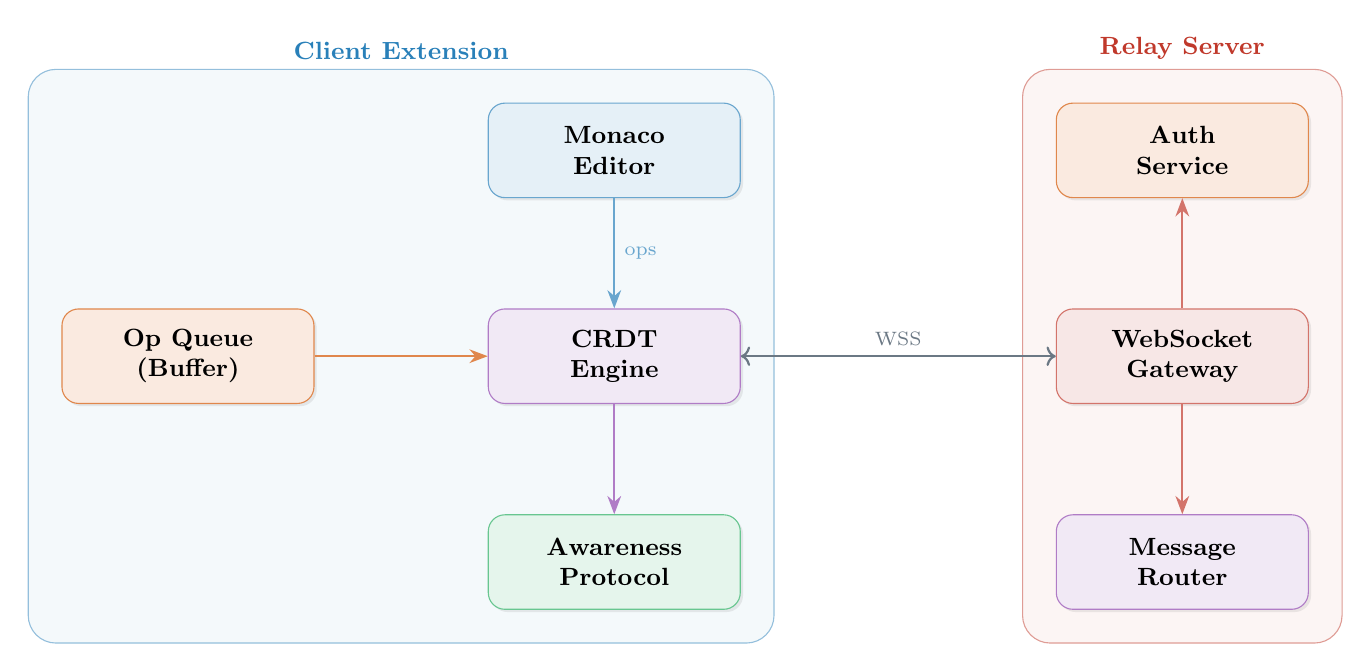
\begin{tikzpicture}[node distance=1.4cm and 1.6cm]

  % Client-Side
  \node[component=client] (editor) {Monaco\\Editor};
  \node[component=crdt, below=of editor] (crdtlocal) {CRDT\\Engine};
  \node[component=accentgreen, below=of crdtlocal] (awareness) {Awareness\\Protocol};
  \node[component=broker, left=2.2cm of crdtlocal] (queue) {Op Queue\\(Buffer)};

  % Background
  \begin{scope}[on background layer]
    \node[fit=(editor)(crdtlocal)(awareness)(queue),
          rectangle, rounded corners=10pt, draw=client!50, fill=client!5,
          inner sep=12pt, label={[font=\small\bfseries\color{client}]above:Client Extension}] (clientbox) {};
  \end{scope}

  % Network
  \node[component=server, right=4cm of crdtlocal] (ws) {WebSocket\\Gateway};
  \node[component=broker, above=of ws] (auth) {Auth\\Service};
  \node[component=crdt, below=of ws] (router) {Message\\Router};

  \begin{scope}[on background layer]
    \node[fit=(ws)(auth)(router),
          rectangle, rounded corners=10pt, draw=server!50, fill=server!5,
          inner sep=12pt, label={[font=\small\bfseries\color{server}]above:Relay Server}] (serverbox) {};
  \end{scope}

  % Arrows
  \draw[connector=client] (editor) -- node[right, font=\scriptsize]{ops} (crdtlocal);
  \draw[connector=crdt] (crdtlocal) -- (awareness);
  \draw[connector=broker] (queue) -- (crdtlocal);
  \draw[connector=primaryblue, <->] (crdtlocal.east) -- node[above, font=\scriptsize]{WSS} (ws.west);
  \draw[connector=server] (ws) -- (auth);
  \draw[connector=server] (ws) -- (router);

\end{tikzpicture}
}
\caption{Component Decomposition --- Internal Services}
\label{fig:components}
\end{figure}

\subsection{Communication Protocol Sequence}

% --- SEQUENCE DIAGRAM ---
\begin{figure}[H]
\centering
\resizebox{0.95\textwidth}{!}{
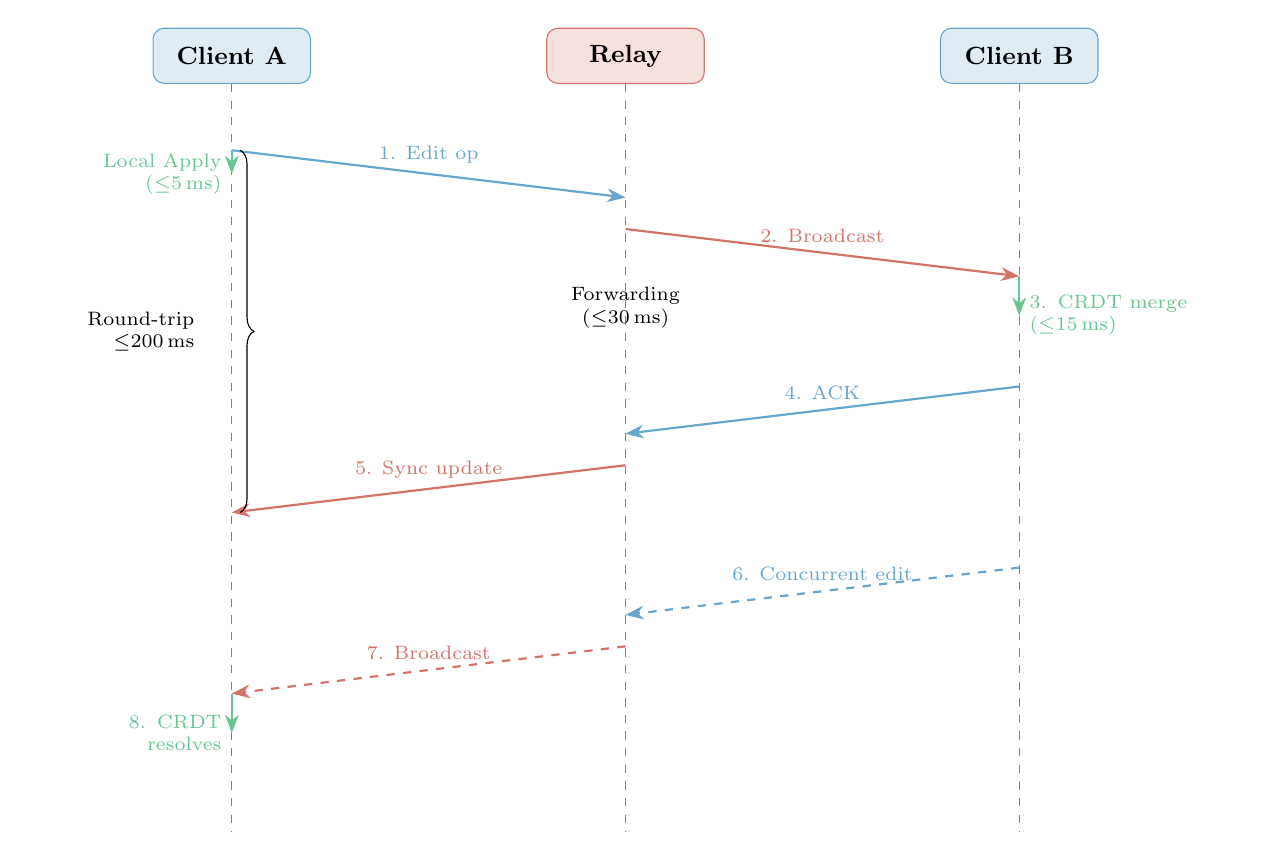
\begin{tikzpicture}[
  actor/.style={rectangle, rounded corners=4pt, minimum width=2cm, minimum height=0.7cm,
                draw=#1!70, fill=#1!15, font=\small\bfseries, align=center},
  msg/.style={-Stealth, thick, color=#1!70},
]
  % Actors
  \node[actor=client] (A) at (0,0) {Client A};
  \node[actor=server] (S) at (5,0) {Relay};
  \node[actor=client] (B) at (10,0) {Client B};

  % Lifelines
  \draw[dashed, gray] (A.south) -- ++(0,-9.5);
  \draw[dashed, gray] (S.south) -- ++(0,-9.5);
  \draw[dashed, gray] (B.south) -- ++(0,-9.5);

  % Messages
  \draw[msg=client] (0,-1.2) -- node[above, font=\scriptsize]{1. Edit op} (5,-1.8);
  \draw[msg=accentgreen] (0,-1.2) -- ++(0,-0.3) node[left, font=\scriptsize, text width=2.2cm, align=right]{Local Apply\\($\leq$5\,ms)};

  \draw[msg=server] (5,-2.2) -- node[above, font=\scriptsize]{2. Broadcast} (10,-2.8);
  \node[font=\scriptsize, text width=2cm, align=center] at (5,-3.2) {Forwarding\\($\leq$30\,ms)};

  \draw[msg=accentgreen] (10,-2.8) -- ++(0,-0.5) node[right, font=\scriptsize, text width=2.5cm]{3. CRDT merge\\($\leq$15\,ms)};

  \draw[msg=client] (10,-4.2) -- node[above, font=\scriptsize]{4. ACK} (5,-4.8);
  \draw[msg=server] (5,-5.2) -- node[above, font=\scriptsize]{5. Sync update} (0,-5.8);

  % Concurrent edit
  \draw[msg=client, dashed] (10,-6.5) -- node[above, font=\scriptsize]{6. Concurrent edit} (5,-7.1);
  \draw[msg=server, dashed] (5,-7.5) -- node[above, font=\scriptsize]{7. Broadcast} (0,-8.1);
  \draw[msg=accentgreen] (0,-8.1) -- ++(0,-0.5) node[left, font=\scriptsize, text width=2.2cm, align=right]{8. CRDT resolves};

  % Timing annotation
  \draw[decorate, decoration={brace, amplitude=5pt, raise=3pt}]
    (0,-1.2) -- (0,-5.8) node[midway, left=10pt, font=\scriptsize, text width=2cm, align=right]
    {Round-trip\\$\leq$200\,ms};

\end{tikzpicture}
}
\caption{System Synchronization Sequence}
\label{fig:sequence}
\end{figure}

\subsection{Consistency Model}

\begin{figure}[H]
\centering
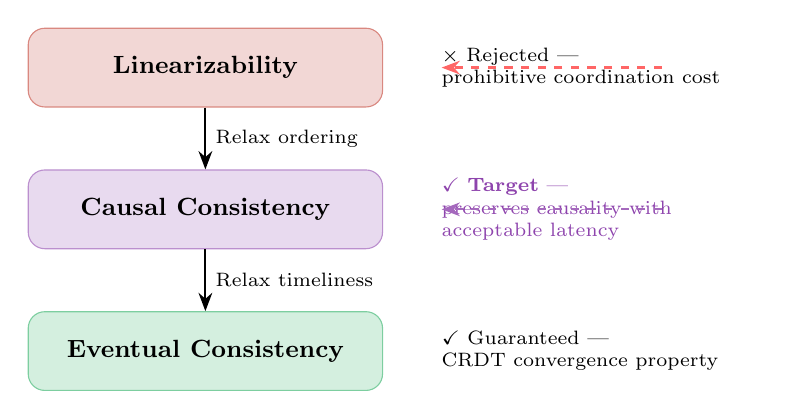
\begin{tikzpicture}[
  level/.style={rectangle, rounded corners=6pt, minimum width=4.5cm, minimum height=1cm,
                align=center, font=\small\bfseries},
]
  \node[level, fill=server!20, draw=server!60] (linear) at (0,0) {Linearizability};
  \node[level, fill=crdt!20, draw=crdt!60] (causal) at (0,-1.8) {Causal Consistency};
  \node[level, fill=accentgreen!20, draw=accentgreen!60] (eventual) at (0,-3.6) {Eventual Consistency};

  \draw[-Stealth, thick] (linear.south) -- node[right, font=\scriptsize]{Relax ordering} (causal.north);
  \draw[-Stealth, thick] (causal.south) -- node[right, font=\scriptsize]{Relax timeliness} (eventual.north);

  \node[font=\scriptsize, text width=4cm, align=left] at (5, 0) {$\times$ Rejected ---\\prohibitive coordination cost};
  \node[font=\scriptsize, text width=4cm, align=left, color=crdt] at (5,-1.8) {$\checkmark$ \textbf{Target} ---\\preserves causality with\\acceptable latency};
  \node[font=\scriptsize, text width=4cm, align=left] at (5,-3.6) {$\checkmark$ Guaranteed ---\\CRDT convergence property};

  \draw[-Stealth, dashed, red!60, thick] (5.8,0) -- (3,0);
  \draw[-Stealth, dashed, crdt!80, thick] (5.8,-1.8) -- (3,-1.8);

\end{tikzpicture}
\caption{Consistency Model Hierarchy --- CollabCode targets Causal Consistency with Eventual Consistency as the convergence guarantee.}
\label{fig:consistency}
\end{figure}

\subsection{CRDT vs.\ OT Trade-off Analysis}

\begin{table}[H]
\centering
\caption{Architectural Decision: CRDT vs.\ OT}
\begin{tabularx}{\textwidth}{l X X}
\toprule
\textbf{Criterion} & \textbf{OT (e.g., Google Docs)} & \textbf{CRDT (e.g., Yjs)} \\
\midrule
Central server required & Yes (sequencing) & No (peer-to-peer capable) \\
Correctness proof complexity & High (TP1/TP2 conditions) & Moderate (mathematical commutativity) \\
Offline editing support & Limited & Native \\
Memory overhead per character & Low ($\sim$1 byte) & Higher ($\sim$4--8 bytes metadata) \\
Merge determinism & Transform-dependent & Guaranteed by algebraic properties \\
Library maturity & ShareJS (unmaintained) & \textbf{Yjs}, Automerge (active) \\
\midrule
\multicolumn{3}{l}{\textbf{Decision:} \textcolor{crdt}{\textbf{CRDT (Yjs)}} --- superior offline support, no central sequencer, proven library.} \\
\bottomrule
\end{tabularx}
\end{table}

% ===================== 6. ATAM SCENARIOS =====================
\section{Architecture Evaluation --- ATAM Scenarios}

The Architecture Tradeoff Analysis Method (ATAM) is applied to six high-priority scenarios. Each scenario maps a stimulus to an architectural response and a measurable metric.

\begin{table}[H]
\centering
\caption{ATAM Scenarios and Evaluations}
\resizebox{\textwidth}{!}{
\begin{tabularx}{1.1\textwidth}{c l Y Y c}
\toprule
\textbf{\#} & \textbf{QA} & \textbf{Scenario} & \textbf{Architectural Response} & \textbf{Measure} \\
\midrule
1 & Perf. & Two users type on same line. & CRDT resolves at each replica. & $\leq$200\,ms \\
\addlinespace
2 & Rel. & Client B loses network for 45\,s. & Ops queued locally; CRDT sync on reconnect. & 0 lost \\
\addlinespace
3 & Perf. & 8 users in different files. & Multiplexed per-doc channels; independent CRDT. & $\leq$250\,ms \\
\addlinespace
4 & Sec. & Unauthorized join attempt. & 128-bit session token; 5 joins/min rate limit. & $\approx 0$ \\
\addlinespace
5 & Usab. & New user start-to-finish. & Guided onboarding; dedicated start command. & $\leq$120\,s \\
\addlinespace
6 & Scal. & 500\,KB doc / 200K ops. & Periodic GC compacts metadata; snapshots. & $\leq$150\,MB \\
\bottomrule
\end{tabularx}
}
\end{table}

% --- ATAM UTILITY TREE ---
\begin{figure}[H]
\centering
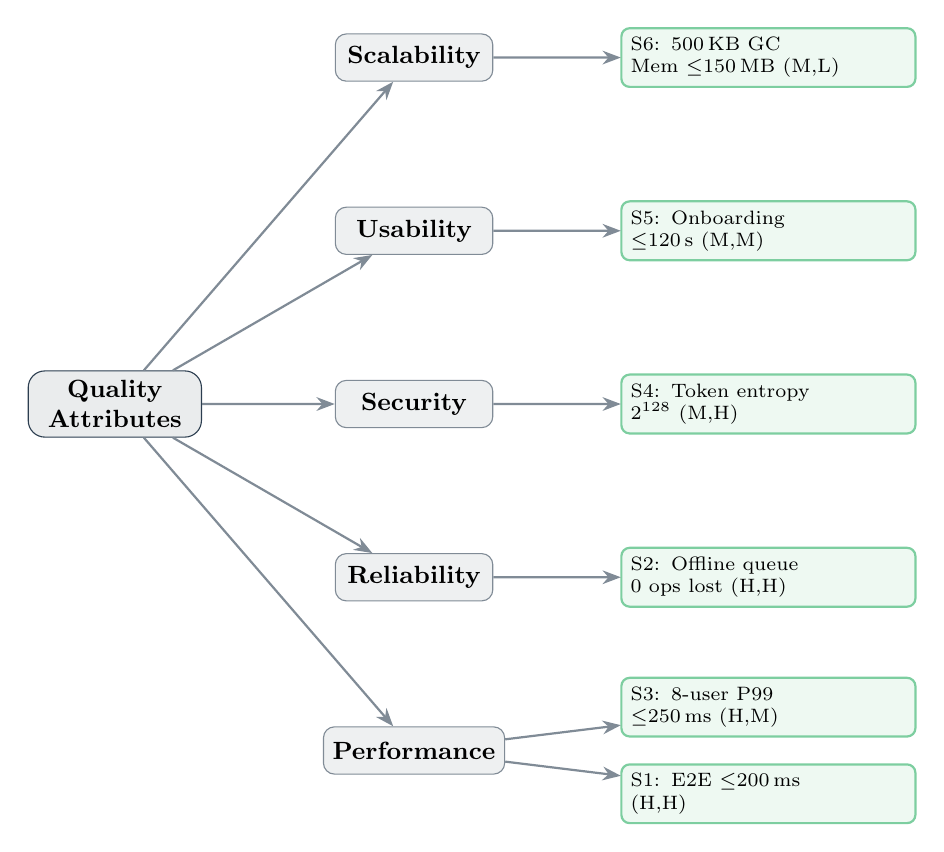
\begin{tikzpicture}[
  grow=right,
  level 1/.style={sibling distance=2.2cm, level distance=3.8cm},
  level 2/.style={sibling distance=1.1cm, level distance=4.5cm},
  every node/.style={font=\small},
  edge from parent/.style={draw, -Stealth, thick, primaryblue!60},
  root/.style={rectangle, rounded corners=6pt, draw=sectioncolor, fill=sectioncolor!10,
               font=\small\bfseries, minimum width=2.2cm, minimum height=0.8cm, align=center},
  qa/.style={rectangle, rounded corners=4pt, draw=primaryblue!60, fill=primaryblue!8,
             font=\small\bfseries, minimum width=2cm, minimum height=0.6cm, align=center},
  scenario/.style={rectangle, rounded corners=3pt, draw=accentgreen!60, fill=accentgreen!8,
                   font=\scriptsize, text width=3.5cm, align=left},
]
  \node[root] {Quality\\Attributes}
    child { node[qa] {Performance}
      child { node[scenario] {S1: E2E $\leq$200\,ms\\(H,H)} }
      child { node[scenario] {S3: 8-user P99\\$\leq$250\,ms (H,M)} }
    }
    child { node[qa] {Reliability}
      child { node[scenario] {S2: Offline queue\\0 ops lost (H,H)} }
    }
    child { node[qa] {Security}
      child { node[scenario] {S4: Token entropy\\$2^{128}$ (M,H)} }
    }
    child { node[qa] {Usability}
      child { node[scenario] {S5: Onboarding\\$\leq$120\,s (M,M)} }
    }
    child { node[qa] {Scalability}
      child { node[scenario] {S6: 500\,KB GC\\Mem $\leq$150\,MB (M,L)} }
    };
\end{tikzpicture}
\caption{ATAM Utility Tree --- (Importance, Difficulty) ratings per scenario. H=High, M=Medium, L=Low.}
\label{fig:utility}
\end{figure}

% ===================== 7. FAILURE MODE ANALYSIS =====================
\section{Failure Mode Analysis}

% --- FAILURE SCENARIO DIAGRAM ---
\begin{figure}[H]
\centering
\resizebox{0.9\textwidth}{!}{
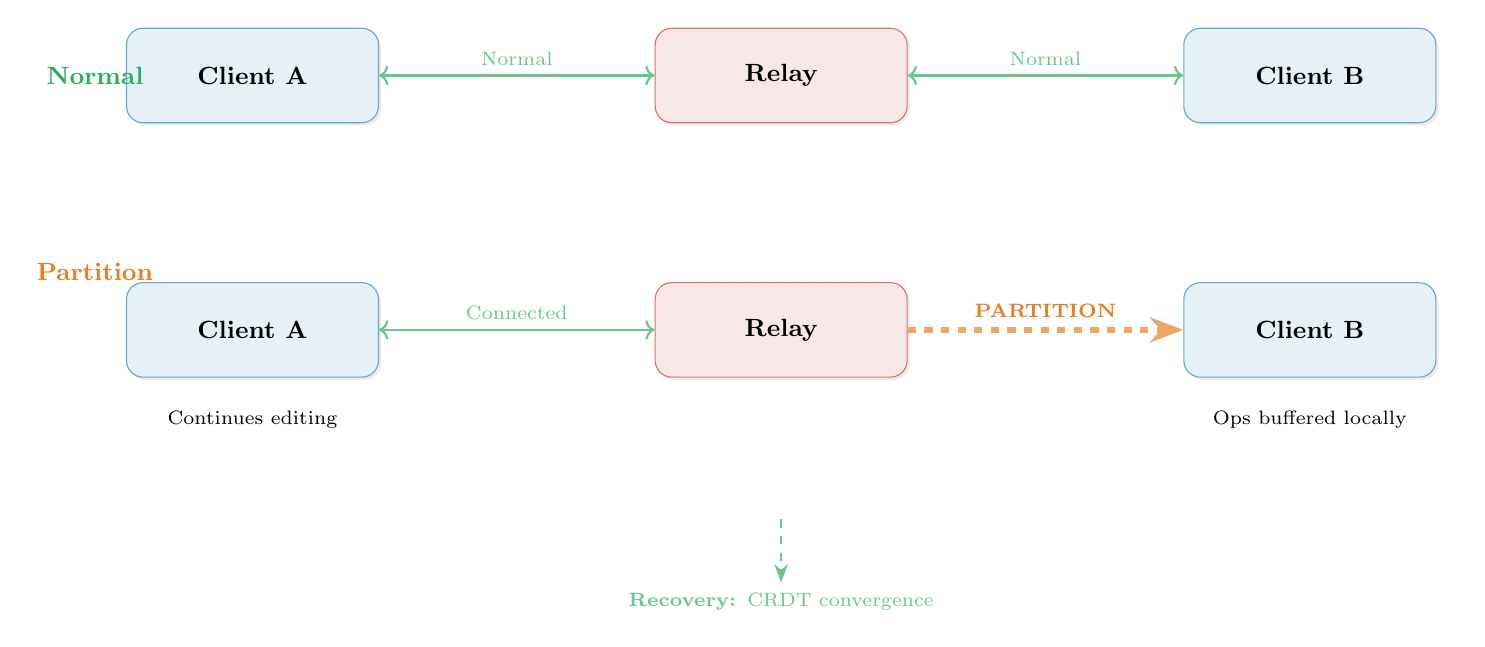
\begin{tikzpicture}[node distance=1.2cm and 2.5cm]

  \node[component=client] (ca) {Client A};
  \node[component=server, right=3.5cm of ca] (relay) {Relay};
  \node[component=client, right=3.5cm of relay] (cb) {Client B};

  % Normal flow
  \draw[connector=accentgreen, <->] (ca) -- node[above, font=\scriptsize]{Normal} (relay);
  \draw[connector=accentgreen, <->] (relay) -- node[above, font=\scriptsize]{Normal} (cb);

  % Failure: network partition
  \node[below=2.5cm of relay] (fail) {};
  \node[component=client] (ca2) at (ca |- fail) {Client A};
  \node[component=server] (relay2) at (relay |- fail) {Relay};
  \node[component=client] (cb2) at (cb |- fail) {Client B};

  \draw[connector=accentgreen, <->] (ca2) -- node[above, font=\scriptsize]{Connected} (relay2);
  \draw[connector=warnorange, dashed, line width=2pt] (relay2) -- node[above, font=\scriptsize, color=warnorange]{\textbf{PARTITION}} (cb2);

  % Recovery
  \node[font=\scriptsize, text width=3.5cm, align=center, below=0.3cm of cb2]
    {Ops buffered locally};
  \node[font=\scriptsize, text width=3.5cm, align=center, below=0.3cm of ca2]
    {Continues editing};

  % Arrow showing recovery
  \draw[-Stealth, thick, accentgreen!70, dashed]
    ([yshift=-1.8cm]relay2.south) -- ++(0,-0.8)
    node[below, font=\scriptsize, text width=4cm, align=center]
    {\textbf{Recovery:} CRDT convergence};

  % Labels
  \node[font=\small\bfseries\color{accentgreen}] at (-2, 0) {Normal};
  \node[font=\small\bfseries\color{warnorange}] at (-2, -2.5) {Partition};

\end{tikzpicture}
}
\caption{Failure Scenario and Recovery Logic}
\label{fig:failure}
\end{figure}

\begin{table}[H]
\centering
\caption{Failure Modes and Mitigation Strategies}
\begin{tabularx}{\textwidth}{l X X c}
\toprule
\textbf{Failure Mode} & \textbf{Impact} & \textbf{Mitigation} & \textbf{Recovery} \\
\midrule
Network partition & Replicas diverge temporarily & Local op queue + CRDT convergence on reconnect & $\leq$500\,ms \\
Relay server crash & No new message routing & Auto-restart (container); clients buffer ops & $\leq$30\,s \\
Out-of-order messages & Potential inconsistency & Causal ordering via vector clocks in CRDT & Automatic \\
Client crash & Unsaved CRDT state lost & Periodic local snapshot every 10\,s & $\leq$10\,s data loss \\
Token interception & Unauthorized session access & TLS 1.3 + token expiry (24\,hr) + PKCE & Immediate \\
\bottomrule
\end{tabularx}
\end{table}

% ===================== 8. WALKING SKELETON =====================
\section{Walking Skeleton Plan}

The walking skeleton validates the highest-risk architectural element: \textbf{real-time CRDT synchronization across two IDE instances}.

\begin{table}[H]
\centering
\caption{Walking Skeleton --- Sprint Plan}
\begin{tabularx}{\textwidth}{c c X X}
\toprule
\textbf{Sprint} & \textbf{Duration} & \textbf{Deliverables} & \textbf{Validation Criteria} \\
\midrule
1 & Weeks 1--4 & Walking skeleton: 2-client text sync via Yjs + WebSocket relay & Concurrent edits converge with 100\% consistency; E2E $\leq$200\,ms \\
2 & Weeks 5--8 & Presence awareness, session management, basic auth, multi-file support & Live cursors update at $\geq$10\,Hz; session join $\leq$2\,s \\
3 & Weeks 9--12 & Shared terminal, chat, polish, ATAM evaluation, performance benchmarks & All NFRs met; SUS score $\geq$72; ATAM report complete \\
\bottomrule
\end{tabularx}
\end{table}

% ===================== 9. VALIDATION METRICS =====================
\section{Verification and Validation Plan}

\subsection{Quantified Acceptance Criteria}

\begin{table}[H]
\centering
\caption{Validation Metrics and Acceptance Thresholds}
\begin{tabularx}{\textwidth}{l X c c c}
\toprule
\textbf{ID} & \textbf{Metric} & \textbf{Tool} & \textbf{Pass} & \textbf{Fail} \\
\midrule
VM-01 & E2E latency P95 & Custom benchmarks & $\leq$150\,ms & $>$200\,ms \\
VM-02 & Convergence rate (10K concurrent ops) & Automated test harness & 100\% & $<$100\% \\
VM-03 & Throughput (ops/sec, 8 users) & Load generator & $\geq$500 & $<$200 \\
VM-04 & Memory footprint (client, 500\,KB doc) & Chrome DevTools & $\leq$150\,MB & $>$200\,MB \\
VM-05 & Defect Miss Rate (DMR) & CI/CD test suite & $\leq$2\% & $>$5\% \\
VM-06 & SUS Usability Score & User survey ($n\geq 8$) & $\geq$72 & $<$60 \\
VM-07 & Offline queue resilience & Chaos testing (network kill) & 0 ops lost & Any loss \\
VM-08 & Security pen-test (token brute-force) & Automated scanner & 0 breaches & Any breach \\
\bottomrule
\end{tabularx}
\end{table}

\subsection{Testing Strategy}

% --- TESTING PYRAMID ---
\begin{figure}[H]
\centering
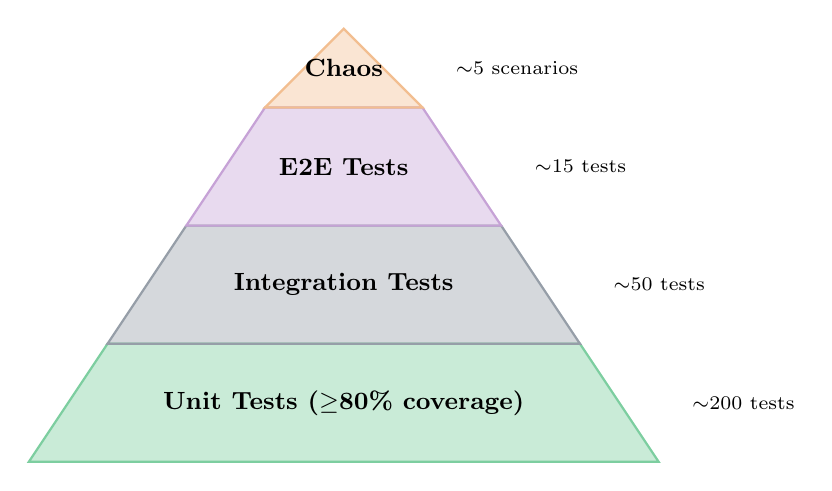
\begin{tikzpicture}
  % Pyramid layers
  \fill[accentgreen!25] (-4,0) -- (4,0) -- (3,1.5) -- (-3,1.5) -- cycle;
  \fill[primaryblue!20] (-3,1.5) -- (3,1.5) -- (2,3) -- (-2,3) -- cycle;
  \fill[crdt!20] (-2,3) -- (2,3) -- (1,4.5) -- (-1,4.5) -- cycle;
  \fill[warnorange!20] (-1,4.5) -- (1,4.5) -- (0,5.5) -- cycle;

  % Borders
  \draw[accentgreen!60, thick] (-4,0) -- (4,0) -- (3,1.5) -- (-3,1.5) -- cycle;
  \draw[primaryblue!50, thick] (-3,1.5) -- (3,1.5) -- (2,3) -- (-2,3) -- cycle;
  \draw[crdt!50, thick] (-2,3) -- (2,3) -- (1,4.5) -- (-1,4.5) -- cycle;
  \draw[warnorange!50, thick] (-1,4.5) -- (1,4.5) -- (0,5.5) -- cycle;

  % Labels
  \node[font=\small\bfseries] at (0, 0.75) {Unit Tests ($\geq$80\% coverage)};
  \node[font=\small\bfseries] at (0, 2.25) {Integration Tests};
  \node[font=\small\bfseries] at (0, 3.75) {E2E Tests};
  \node[font=\small\bfseries] at (0, 5.0) {Chaos};

  % Counts
  \node[font=\scriptsize, right] at (4.3, 0.75) {$\sim$200 tests};
  \node[font=\scriptsize, right] at (3.3, 2.25) {$\sim$50 tests};
  \node[font=\scriptsize, right] at (2.3, 3.75) {$\sim$15 tests};
  \node[font=\scriptsize, right] at (1.3, 5.0) {$\sim$5 scenarios};

\end{tikzpicture}
\caption{Testing Pyramid --- Test distribution by granularity.}
\label{fig:testing}
\end{figure}

% ===================== 10. TRACEABILITY MATRIX =====================
\section{Requirements Traceability Matrix}

\begin{table}[H]
\centering
\caption{Requirements Traceability Matrix}
\begin{tabularx}{\textwidth}{l Y Y c}
\toprule
\textbf{Requirement} & \textbf{Component} & \textbf{Test ID} & \textbf{ATAM} \\
\midrule
FR-CE-01 (Local) & CRDT Engine & VM-01, VM-03 & S1 \\
FR-CE-03 (Conflict) & CRDT Engine & VM-02 & S1, S2 \\
FR-SM-02 (Join) & WebSocket Gateway & VM-01, VM-07 & S5 \\
FR-PA-01 (Cursors) & Awareness Protocol & VM-01 & S3 \\
NFR-P-01 (Latency) & All client + relay & VM-01 & S1, S3 \\
NFR-R-02 (Convergence) & CRDT Engine & VM-02, VM-07 & S2 \\
NFR-S-02 (Token) & Auth Service & VM-08 & S4 \\
NFR-SC-01 (8 users) & Relay, Router & VM-03, VM-04 & S3, S6 \\
\bottomrule
\end{tabularx}
\end{table}

% ===================== 11. GLOSSARY =====================
\section{Glossary}
\begin{description}[style=nextline, leftmargin=3cm]
  \item[Convergence] The property that all replicas eventually reach an identical state after all operations are delivered.
  \item[Leader] A node authorized to accept writes; in multi-leader replication, every node is a leader.
  \item[Operation (Op)] A single atomic edit action (insert, delete) encoded for network transmission.
  \item[Replica] A local copy of the shared document state maintained at each client.
  \item[State Vector] A compact representation of a CRDT node's knowledge of all operations it has observed.
  \item[Vector Clock] A mechanism for tracking causal ordering of events across distributed nodes.
  \item[Walking Skeleton] A minimal, end-to-end implementation that exercises the system's core architectural path.
\end{description}

% ===================== APPENDIX =====================
\appendix
\section{Technology Stack}
\begin{table}[H]
\centering
\begin{tabularx}{\textwidth}{l l X}
\toprule
\textbf{Layer} & \textbf{Technology} & \textbf{Rationale} \\
\midrule
CRDT Library & Yjs v13+ & Most mature JS CRDT; sub-ms local merge; Awareness protocol built-in \\
Transport & ws (Node.js) & Lightweight WebSocket server; $<$5\,ms overhead per message \\
Client Framework & VS Code Extension API & Native integration with Monaco editor and extension marketplace \\
Server Runtime & Node.js 20 LTS & Event-loop model ideal for I/O-bound relay workload \\
Containerization & Docker + Compose & Reproducible deployment; easy CI/CD integration \\
Auth & OAuth 2.0 + PKCE & Industry-standard; no client-secret exposure \\
Testing & Vitest + Playwright & Fast unit tests + browser-level E2E for multi-client scenarios \\
\bottomrule
\end{tabularx}
\end{table}

\section{Estimated Effort Breakdown}
\begin{table}[H]
\centering
\begin{tabularx}{\textwidth}{X c c c}
\toprule
\textbf{Work Package} & \textbf{Estimated Hours} & \textbf{Team Members} & \textbf{Sprint} \\
\midrule
CRDT integration + relay server & 120 & 2 & 1 \\
VS Code extension scaffolding & 60 & 1 & 1 \\
Session management + auth & 80 & 2 & 1--2 \\
Presence awareness (cursors, selections) & 60 & 1 & 2 \\
Multi-file support + file tree sync & 50 & 1 & 2 \\
Shared terminal + debugging proxy & 80 & 2 & 3 \\
Chat + annotations & 30 & 1 & 3 \\
Testing infrastructure + benchmarks & 70 & 2 & 1--3 \\
ATAM evaluation + documentation & 40 & 1 & 3 \\
\midrule
\textbf{Total} & \textbf{590 person-hours} & & \\
\bottomrule
\end{tabularx}
\end{table}

\vfill
\begin{center}
\textcolor{gray}{\rule{0.6\textwidth}{0.5pt}}\\[6pt]
{\small\textcolor{sectioncolor}{--- End of Document ---}}
\end{center}

\end{document}
